\documentclass[10pt]{beamer}
\usetheme{Madrid}
\usecolortheme{default}
\setbeamertemplate{navigation symbols}{}

% Packages
\usepackage[utf8]{inputenc}
\usepackage{graphicx}
\usepackage{amsmath}
\usepackage{amsfonts}
\usepackage{amssymb}
\usepackage{xcolor}
\usepackage{tikz}
\usepackage{pgfplots}
\pgfplotsset{compat=1.18}
\usetikzlibrary{arrows,shapes,positioning}

% (Removed listings/code styling to keep slides code-free)

% Title page information
\title[Robot Localization with ROS]{\texorpdfstring{Robot Localization with ROS: \\EKF-based Sensor Fusion Implementation}{Robot Localization with ROS: EKF-based Sensor Fusion Implementation}}
\subtitle{Mini-Project 1 Progress Report}
\author{Nicholas Birch de la Calle (IST1116701) \\
Antonio Maria Trigueiros de Arag\~{a}o Moura Coutinho (IST196837) \\
Gabriel Badan (IST1116537) \\
Jana\'{\i}na da Silva Pacheco (IST1117233)}
\institute{Instituto Superior Técnico}
\date{September 18, 2025}

% Title graphic (IST/Técnico logo). Tries a few common filenames; skips if not found.
\IfFileExists{Tecnico Lisbon Logo.jpg}{\titlegraphic{\includegraphics[height=1.2cm]{Tecnico Lisbon Logo.jpg}}}{%
\IfFileExists{tecnico.jpg}{\titlegraphic{\includegraphics[height=1.2cm]{tecnico.jpg}}}{%
\IfFileExists{logo.jpg}{\titlegraphic{\includegraphics[height=1.2cm]{logo.jpg}}}{}}}

\begin{document}

% Title slide
\begin{frame}
\titlepage
\end{frame}

% Outline
\begin{frame}{Outline}
\tableofcontents
\end{frame}

% Team & scope first
\section{Team \& Scope}

\begin{frame}{Team Workflow \& Scope for This Week}
\begin{itemize}
    \item All teammates use macOS; VMs made Wi-Fi connection to the robot tricky.
    \item We split work to move faster:
    \begin{itemize}
        \item \textbf{Group A:} Fix connectivity to the real robot (prep for mapping in Step 2).
        \item \textbf{Group B:} Use the dataset (.bag) and implement Step 1 (EKF with \texttt{robot\_localization}).
    \end{itemize}
    \item Collaboration: shared notes, common checklist, quick pair-debug sessions on TF and timing.
    \item \textbf{This presentation:} Focus on Step 1 progress with the dataset. Step 2 will follow next week.
\end{itemize}
\end{frame}

% Project overview next
\section{Project Overview}

\begin{frame}{Project Objectives}
\begin{block}{Main Goal}
Implement and test robot self-localization using Extended Kalman Filter (EKF) based localization with ROS \texttt{robot\_localization} package
\end{block}

\begin{itemize}
    \item \textbf{Platform:} TurtleBot3 Waffle Pi with real sensor data
    \item \textbf{Sensors:} IMU, wheel odometry, laser scanner
    \item \textbf{Method:} EKF-based sensor fusion
    \item \textbf{Data:} Pre-recorded rosbags with ground truth from Motion Capture System
    \item \textbf{Framework:} ROS Noetic environment
\end{itemize}

\begin{alertblock}{Key Learning Outcomes}
Understanding Bayesian filtering, ROS navigation stack, and practical sensor fusion implementation
\end{alertblock}
\end{frame}

\begin{frame}{Dataset Information}
\begin{columns}
\begin{column}{0.6\textwidth}
    	\textbf{What’s inside:}
\begin{itemize}
    \item Wheel odometry (\texttt{/odom})
    \item IMU measurements (\texttt{/imu})
    \item Laser scans (\texttt{/scan})
    \item Ground truth in TF (\texttt{mocap} but not used this week yet)
    \item Camera topics are present but not used this week
\end{itemize}
\vspace{0.2cm}
\scriptsize Dataset source: \url{https://github.com/irob-labs-ist/turtlebot3_datasets}\\
\scriptsize This week we did not use the helper TF script and we did not compare to mocap yet.
\end{column}
\begin{column}{0.4\textwidth}
\begin{center}
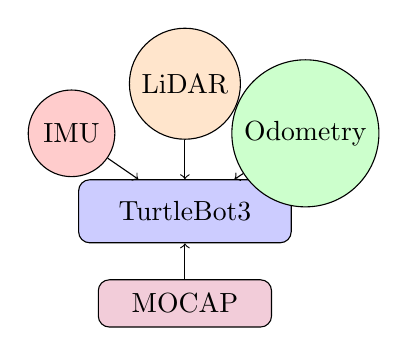
\begin{tikzpicture}[scale=0.9]

% Balanced sensor bubbles
\node[draw, rectangle, rounded corners, fill=blue!20, minimum width=2.7cm, minimum height=0.8cm] (robot) at (0,0) {TurtleBot3};
\node[draw, circle, fill=red!20, minimum size=1.1cm] (imu) at (-1.6,1.1) {IMU};
    \node[draw, circle, fill=green!20, minimum size=0.9cm] (odom) at (1.7,1.1) {Odometry};
\node[draw, circle, fill=orange!20, minimum size=1.1cm] (lidar) at (0,1.8) {LiDAR};
\node[draw, rectangle, rounded corners, fill=purple!20, minimum width=2.2cm, minimum height=0.6cm] (mocap) at (0,-1.3) {MOCAP};

\draw[->] (imu) -- (robot);
\draw[->] (odom) -- (robot);
\draw[->] (lidar) -- (robot);
\draw[->] (mocap) -- (robot);
\end{tikzpicture}
\end{center}
\end{column}
\end{columns}
\end{frame}

% Duplicate Team & Scope slide removed

% (Slides 6–8 removed as requested)

% (Slide removed as requested)

% Removed duplicate "How We Ran It" slide

% Section 4: Technical Challenges
% (Section and slide removed as requested)

% (Diagnostics slide removed to keep things simple)

% Section 5: Current Status
\section{Status \& What’s Next}

\begin{frame}{Status and Next Steps}
\begin{itemize}
    \item \textbf{Status:} EKF running on the dataset; we compared \texttt{/odom} (orange) vs \texttt{/odometry/filtered} (red) in RViz.
    \item \textbf{Observation:} There is a small, slow drift between the two trajectories.
    \item \textbf{Next:} Extract mocap ground-truth trajectory and quantitatively compare against both.
    \item \textbf{Coming up:} Map-based trajectory comparison and gmapping with the real robot (Step 2).
\end{itemize}
\end{frame}

% (Slide removed as requested)

% RViz itineraries slide
\begin{frame}{RViz Trajectory Comparison}
\begin{itemize}
    \item \textbf{Fixed Frame:} \texttt{odom}.
    \item \textbf{Odometry (orange):} \texttt{/odom}
    \item \textbf{Filtered odometry (red):} \texttt{/odometry/filtered}
    \item We did not use the map-based trajectory yet, that’s for next week.
    \item We can see a slow drift between the two. To know which is more accurate, we’ll extract the mocap ground-truth trajectory next week and compare.
\end{itemize}
\begin{center}
\includegraphics[width=0.9\textwidth]{image.png}
\\[2mm]
\scriptsize (RViz screenshot: orange = /odom, red = /odometry/filtered)
\end{center}
\end{frame}

% (Detailed evaluation plan removed; will present once IMU is integrated)

% Section 6: Conclusion
% (Section and slide removed as requested)

% (Extra theory slide removed to keep it accessible)

\begin{frame}{Final Remarks}
\begin{block}{Progress Summary}
Successfully established a working EKF setup with visual comparison between odometry and filtered odometry. We kept the analysis simple and focused on Step 1.
\end{block}

\begin{block}{Next Session Goals}
\begin{enumerate}
    \item Extract mocap ground-truth trajectory and align frames
    \item Quantitatively compare mocap vs \texttt{/odom} and \texttt{/odometry/filtered}
    \item Add map-based trajectory comparison
    \item Prepare for Phase 2: SLAM with gmapping
\end{enumerate}
\end{block}

\begin{center}
\Large \textbf{Thank you for your attention!} \\
\vspace{0.5cm}
\normalsize Questions?
\end{center}
\end{frame}

\end{document}